\documentclass[]{article}
\usepackage[T1]{fontenc}
\usepackage[utf8]{inputenc}
\usepackage[swedish]{babel}
\usepackage[backend=biber,style=verbose-ibid,citestyle=authortitle-ibid]{biblatex}
\usepackage{comment}
\usepackage{amsmath,amsfonts}
\usepackage{graphicx}
\usepackage{lmodern,microtype}
\usepackage[dvipsnames,svgnames]{xcolor}
\usepackage{tikz,pgfplots,pgfplotstable}
\usepackage{rotating}
\usepackage{rotfloat}
\usepackage{siunitx}

\bibliography{cites}
\usetikzlibrary{shapes,arrows,intersections,decorations.pathreplacing,calc,quotes,angles,babel,matrix,chains,positioning}
\usepgfplotslibrary{units,groupplots}
\sisetup{
	output-decimal-marker = {,},
	round-mode=figures
}
\DeclareSIUnit\styck{st}

\begin{document}

%\begin{comment}
%försättsblad
\begin{titlepage}
	\centering
	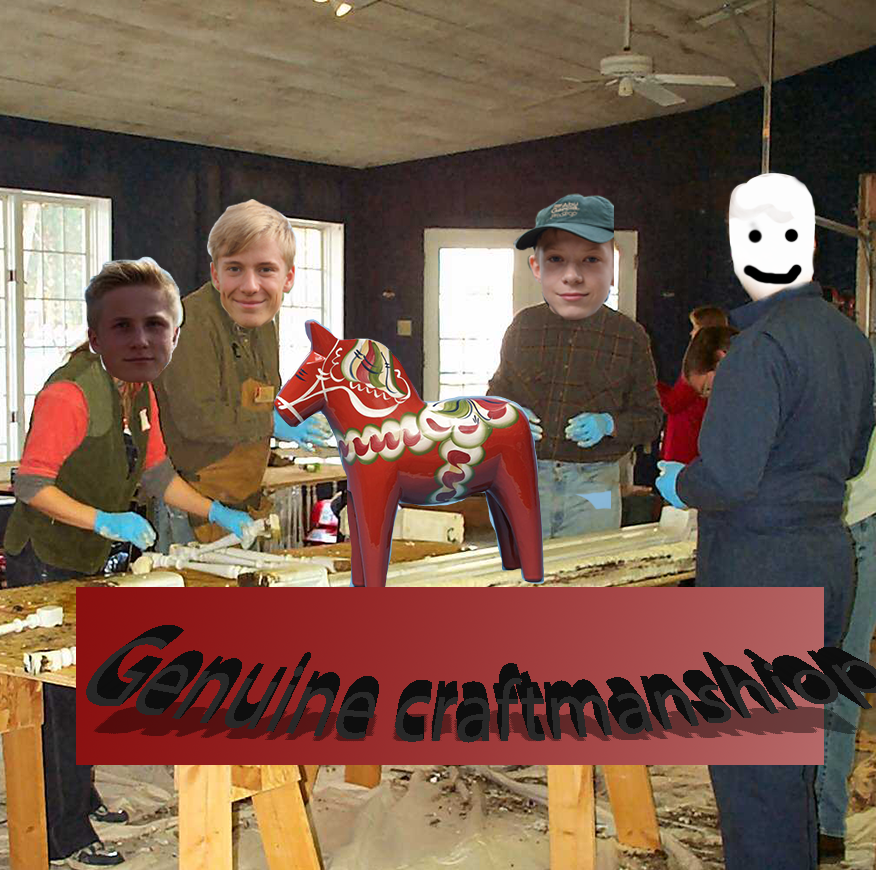
\includegraphics[height=3.5cm]{messengerpicture.png}\par
	\vspace{0.6cm}
	{\scshape\LARGE Hulebäcksgymnasiet}\par
	\vspace{0.5cm}
	{\bfseries\Large Gymnasiearbete}\par
	\vspace{2cm}
	{\scshape\huge Felkompensering av Lutningsgivare med Neuronnät}\par
	\vfill
	{\Large\itshape Anders, Axel, Jonas \& William}\par
	\vspace{0.4cm}
	{\large Handledare: {\itshape Èva Fülöp}}\par
	\vspace{0.4cm}
	{\today\par}
\end{titlepage}

% Innehållsförtecking
\pagenumbering{gobble}
\tableofcontents
\cleardoublepage
\pagenumbering{arabic}
%\end{comment}

%Rapporten
\section{Teori \& bakgrund}
\subsection{Inledning}
% Bakgrund
Automatiska växellådor sitter idag i en mängd av olika fordon,
däribland en helt elektrisk buss under utveckling av Volvo.
För att bland annat köra på rätt växel, optimera motorns styrprogram
och operera olika bromsfunktioner % och vad mer/något mer?
mätes fordonets lutning.
För det ändamålet ska lutningsgivare användas.
Lutningsgivaren är en fristående modul som använder piezokristaller för att
mäta lutningen och kommunicerar med styrdatorn
via Controller Area Network (CAN) kommunikation.
Detta fungerar bra vid rörelse i konstant hastighet
men vid accelereration uppstår mätbrus och andra störningar.
Därför behövs en algoritm för att felkompensera dessa störningar.

% Vad neuronnät är och vad de används till
Ett artificiellt neuronnät är en självlärande algoritm som inspirerats av
hur djurs hjärnor fungerar och kommunicerar.
Neuronnät kan användas för att klara av vissa problem som annars är svårlösta
med konventionella datalogiska metoder.
Ett neuronnät ``lär sig'', precis som vi gör, genom att observera.
Men för att ha avsedd funktion måste de tränas, alltså är arbete med neuronnät
uppdelat i två faser: en inlärningsfas och en tillämpningsfas där nätverket sedan
utför den ämnade uppgiften.
\autocite{copeland16}
Det är möjligt att sedan fortsätta träna nätverket
under användning, men oftast slutar man träna det när resultet är önskvärt.
\autocite{wiki-neuronnat}

\subsubsection{Kortfattad översiktsbild}
Lutningsgivaren baseras på en piezoelektrisk kristall och ger vid användning
upphov till mätbrus och andra störningar i de mätvärden den loggar.
Lutningsgivaren kan inte heller skilja mellan om bussen kör på ett lutat underlag
eller om den accelererar, se sektion~\ref{sec:piezo}.
Därför behövs den data som lutningsgivaren samlar in felkompenseras för att
styrenheten i fordonet ska ha avsedd funktion. Bl.a. för att hjälpa växellådan
bestämma rätt växel och för att operera funktioner som ``automatisk startbroms''.
För att felkompensera används ett neuronnät som består av artificiella
neuroner, se sektion~\ref{sec:neuroner}, vilka är konfigurerade i ett nätverk,
se sektion~\ref{sec:arkitektur}. För att nätverket ska fungera önskvärt måste
det tränas -- i det här fallet med en metod som kallas \emph{stochastic gradient descent},
se sektion~\ref{sec:sdg}.

\subsection{Piezoelektriska kristaller}
\label{sec:piezo}
Piezoelektriska material ger upphov till
elektriska laddningar på deras yta under yttre mekaniskt tryck,
vilket kallas den direkta piezoelektriska effekten.
Det mekaniska arbete som utförs omvandlas till elektricitet, det omvända gäller
också, elektricitet omvandlas till mekaniskt arbete i den omvända
piezoelektriska effekten i vilken kristallen deformeras.
\autocite{electronicdesign2016}
Piezoelektriska lutningsgivare använder elektriska signaler som är
inducerade via den piezoelektriska effekten från en piezoelektrisk kropp
under gravitationskraften från en tyngd.
Vinkeln mellan gravitationskraften och
riktningen på den piezoelektriska kroppens vibration
fås av att man mäter magnituden av kraftkomponenten i vibrationens riktning
och använder geometriska samband mellan dem.
\autocite{chiang00}

Vad lutningsgivaren gör kan efterliknas med att mäta en pendels lutning.
Under acceleration kommer den uppmätta lutningen $\phi$
inte överensstämma med den riktiga lutningen $\alpha$.
Kraften från accelerationen ger upphov till en deviation $\beta$:
$ \phi = \alpha + \beta $, se figur~\ref{fig:pendel}.
Eftersom $\alpha$ är så pass liten är den horisontella $F$-komposanten
ungefär lika med accelerationskraften, $ma$, vilket ger:
\begin{equation}
	\left\{ \begin{aligned}
		F \cdot &\cos \beta = mg \\
		F \cdot &\sin \beta = ma
	\end{aligned} \right.
\end{equation}
\begin{equation}
	\frac{mg}{\cos \beta} \cdot \sin \beta = ma \implies \tan \beta = \frac{a}{g}
\end{equation}
För små vinklar mätta i radianer är $ \tan \beta \approx \beta $.
Därför behövs $ \frac{a}{g} $ subtraheras från lutningsgivarens värde.
Detta är Einsteins allmänna relativitetsteori;
lutningsgivaren kan inte särskilja fordonets acceleration och tyngdaccelerationen.
\autocite{lauri17}

% Figur om pendel och acceleration
\begin{figure}
	\centering
	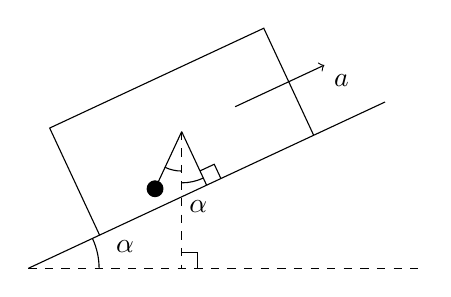
\begin{tikzpicture}
		\begin{scope}[rotate=25]
			\path (2.5, 0.75) coordinate(c) (2.5, 0) coordinate(b);
			\draw (0,0) -- (5, 0) (1, 0) rectangle (4, 1.5) (c) -- (b)
				($ (b) + (0.2, 0) $) |- ($ (b) + (0, 0.2) $);
			\draw[fill] (c) -- +(220:0.8cm) coordinate (p) circle (0.1cm);
			\draw[->] (3.25, 0.75) -- +(1.25,0) node[below right] {$a$};
		\end{scope}
		\path (0, 0) coordinate(o) (c |- o) coordinate(q);
		\draw[dashed] (0,0) -- (5, 0) (c) -- (q);
		\draw ($ (q) + (0.2, 0) $) |- ($ (q) + (0, 0.2) $)
			pic[draw, "$\alpha$", angle radius=0.9cm, angle eccentricity=1.4] {angle = q--o--b}
			pic[draw, angle radius=0.5cm] {angle=p--c--q}
			pic[draw, "$\alpha$", angle radius=0.65cm, angle eccentricity=1.5] {angle = q--c--b};
	\end{tikzpicture}
	\hspace{1cm}
	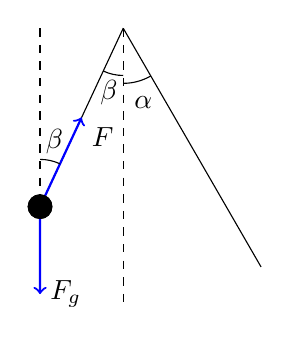
\begin{tikzpicture}
		\coordinate (c) at (4,3.5);
		\draw[fill] (c) -- +(245:2.5cm) coordinate (p) circle (0.15cm);
		\draw[dashed] (c) -- (c |- {0,0}) coordinate (d) (p |- c) coordinate (t) -- (p);
		\draw[<->,draw=blue,thick] ($(p)!0.5!(c)$) node[below right] {$F$} -- (p) -- ($(p)!0.9!(p|-{0,0})$) node[right] {$F_g$};
		\draw (c) -- +(300:3.5cm) coordinate(e)
			pic[draw, "$\alpha$", angle radius=0.7cm, angle eccentricity=1.4] {angle=d--c--e}
			pic[draw, "$\beta$", angle radius=0.6cm, angle eccentricity=1.4] {angle=p--c--d}
			pic[draw, "$\beta$", angle radius=0.6cm, angle eccentricity=1.4] {angle=c--p--t};
		\draw[fill] (p) circle (0.15cm);
	\end{tikzpicture}
	\caption{Pendelanalogin illustrerar hur accelerationen påverkar lutningsgivaren. \label{fig:pendel}}
\end{figure}

% Fel i piezokristaller
Accelerationen orsakar fel i lutningen från lutningsgivaren p.g.a. att
piezokristallernas signal är väldigt svag.
Även när fordonet vibrerar orsakas störningar i signalen och eftersom den är så svag
påverkas den avsevärt.
Sedan finns det ett fel i uppskattningen av accelerationen.
Sensorn som mäter accelerationen använder tidsderivatan av hastigheten för
att räkna ut accelerationen.
Hastigheten mätes via ett kugghjul.
När sensorn i kugghjulet utsätts för viberationer kommer mätningen av
hastigheten att påverkas vilket ger opålitliga resultat.
Detta fel uppstår både vid lutningsapproximation med lutningsgivare likväl som utan.
Dock är felet lättare att lösa när lutningsgivare används.
Dessa anledningar gör att lutningsgivare är fördelaktiga att använda.
\autocite{lauri17}

\subsection{Andra metoder för felkompensering}
\subsubsection{Signalutjämning -- felkompensering utan neuronnät}
Med en lutningsgivare installerad är man inte begränsad till neuronnät för att
felkompensera eftersom att det finns andra metoder, t.ex. signalutjämning.
Instrument kan ge opålitliga värden på grund av eventuella störsignaler.
Ett brus kan visa sig i grafen men det går att minimera bruset med en signalutjämningsfunktion.
Signalutjämningsfunktionen kan se lite olika ut beroende på dess konfiguration
men de har liknande funktion.

En funktionen fungerar så att den använder det nuvarande värdet och
tidigare värden för att hitta ett värde någonstans mellan dem. Vad det
nya värdet blir beror ett värde $c$ vilket säger hur mycket funktionen ska
ta hänsynt till det nuvarande värdet och de tidigare värden. Den enklaste
signalutjämningsfunktionen är förstaordningsfiltret vilket ser ut såhär:
\begin{equation}
	a_{0-new} = a_{0}c + a_{-1}(1 - c)
\end{equation}
Olika värden på $c$ ger olika mycket utjämning på en graf.
I detta fall så ger ett för stort värde av $c$ tillbaka en skakig graf
då förstaordningsfiltret inte anpassar tillräckligt efter det tidigare värdet.
Med ett för litet $c$ kan grafen bli för tillplattad och information förloras.
Det gäller att hitta ett optimalt värde på $c$ för att få en slät graf
utan att förlora för mycket information.

I ett flerordningsfilter så används flera tidigare mätningar för att
beräkna det utslätade värdet av $a_{0}$. Ett flerordningsfilter ser ut såhär:
\begin{equation}
	a_{0-new} = a_{0}c_{1} + a_{-1}c_{2} + \dotsb + a_{1-n}c_{n}
\end{equation}
Där $ c_1 + c_2 + \dotsb + c_n = \sum c = 1 $ för att funktionen
inte ska reducera eller amplifiera värdena.
Flerordningsfilter möjliggör en mer avancerad konfiguration som kan anpassa
nya värden efter mycket äldre värden än det förra värdet som ett
förstaordningsfilter gör.
$c$ kan t.ex anta värdena \{0.2, 0.2, 0.2, 0.2, 0.2\} (med respektive mätvärde
$a_0, a_{-1}, a_{-2}, a_{-3}, a_{-4}$) eller \{0.1, 0.2, 0.3, 0.4\}
(respektive $ a_0, a_{-1}, a_{-2}, a_{-3}$).
Den första konfigurationen skulle ge ett medelvärde över det nya värdet
tillsammans med de fyra tidigare värden. Den andra konfigurationen skulle
inte tillåta det nya mätta värdet att påverka så funktionen så mycket,
utan funktionen lägger större vikt på de tidigare värdena.

%Figur om hur algoritmen fungerar
\begin{figure}
	\centering
	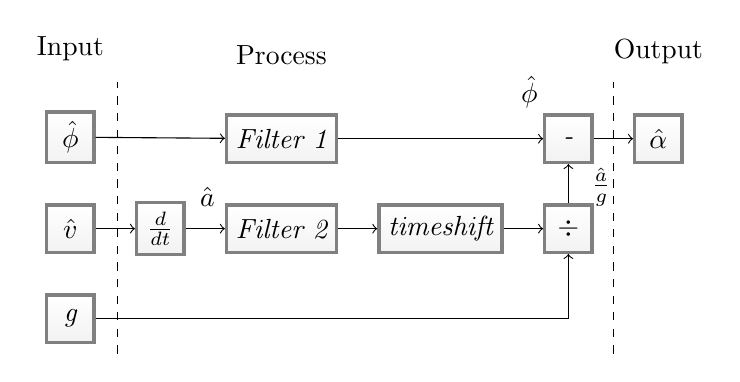
\begin{tikzpicture}[nonterminal/.style={rectangle,minimum size=6mm,very thick,draw=black!50, top color=white, bottom color=black!5, font=\itshape}, node distance=5mm]
		\node (ui1) [nonterminal] {$\hat{\phi }$};
		\node (ui2) [nonterminal,below=of ui1] {$\hat{v}$};
		\node (ui3) [nonterminal,below=of ui2] {g};
		\node (ui4) [above=of ui1] {Input};
		\node (ui7) [nonterminal,right=of ui2] {$ \frac{d}{dt} $};
		\node (ui8) [nonterminal,right=of ui7] {Filter 2};
		\node (ui5) [nonterminal,above=of ui8] {Filter 1};
		\node (ui0) [above= of ui5] {Process};
		\node (ui9) [nonterminal,right=of ui8] {timeshift}; %Timeshiftade vi verkligen?
		\node (ui10) [nonterminal,right=of ui9] {$\div$};
		\node (ui6) [nonterminal,above=of ui10] {-};
		\node (ui11) [nonterminal,right=of ui6] {$\hat{\alpha}$};
		\node (ui12) [above=of ui11] {Output};
		\path (ui1) edge[->] (ui5);
		\path (ui5) edge[->] (ui6) ($(5.7,0.5)!0.5!(5.5,0)$) node[above right] {$\hat{\phi}$};
		\path (ui2) edge[->] (ui7);
		\path (ui7) edge[->] (ui8);
		\path (ui8) edge[->] (ui9);
		\path (ui9) edge[->] (ui10) ($(3.05,-4.0)!0.5!(0,2)$) node[above right] {$\hat{a}$};
		\path (ui10) edge[->] (ui6) ($(6.0,-4.0)!0.5!(7,2)$) node[above right] {$\frac{\hat{a}}{g}$};
		\path (ui6) edge[->] (ui11);
		\draw [->] ($ (ui3.east) $) -| ($ (ui10.south)  $);
		\draw[dashed] (0.6,-2.75) -- (0.6, 0.7);
		\draw[dashed] (6.9,-2.75) -- (6.9, 0.7);
	\end{tikzpicture}
	\caption{Flödesschema för algoritmens struktur. \label{fig:AlgoritmProcess}}
\end{figure}

\subsubsection{Felkompensering utan lutningsgivare}
% Räkna ut lutning med hjälp av moment
Ifall man inte har en lutningsgivare installerad i sitt fordon krävs ändå ett
sätt att räkna ut fordonets lutning.
Detta räknas ut med hjälp av vridmomentet i motorn.
Lutning kan approximeras med god säkerhet vid konstant hastighet men inbromsningar
skapar problem.
Vid inbromsning skapas en friktionskraft som måste tas till hänsyn.
Friktionskraftens moment beräknas med:
\begin{equation}
	M = r \cdot \mu \cdot \lVert F \rVert
\end{equation}
där $F$ är kraften, $r$ är radien i motorns drivaxel, och $\mu$ är friktionskoefficienten
mellan bromsskivan och bromsbeläggen vilken kan variera mellan 0,2 och 0,4.
Därför uppstår en osäkerhet med att räkna ut lutningen utan lutningsgivare.
\autocite{lauri17}

% \subsection{För- och nackdelar med neuronnät}
% \subsubsection{Fördelarna med neuronnät}
% \subsubsection{Nackdelarna med neuronnät}

\subsection{Artificiella neuroner}
\label{sec:neuroner}
% Neuronen
\noindent En artificiell neuron tar in en eller flera inputs och producerar
en output $y$, se figur~\ref{fig:neuron}.
Varje input, $x_n$, är tilldelad en \emph{vikt}, $w_n$.
Utöver det har varje neuron en \emph{bias}, $b$.
Neuronens inputs, $x_1,x_2, \dotsc, x_n$, vikterna, $w_1, w_2, \dotsc, w_n$,
och biasen, $b$, ger en s.k. \emph{weighted input}, $z$:
\begin{equation}
	z \equiv \sum_n w_n x_n + b
\end{equation}
Neuronens output är resultatet av en aktiveringsfunktion för $z$, $\phi(z)$.
Aktiveringsfunktionen kan vara vad som helst så länge den är deriverbar,
men olika funktioner ger olika bra resultat.
Sigmoidfunktionen, $\sigma(z)$, är ett exempel på en sådan aktiveringsfunktion
och ser ut som:
\begin{equation}
	\sigma(z) \equiv \frac{1}{1 + e^{-z}}
\end{equation}
Dess värdemängd är normaliserad från 0\,till\,1, se figur~\ref{fig:sigmoid}.
Om $z$ är ett stort positivt tal kommer $ \sigma(z) \approx 1 $,
medan om $z$ är ett stort negativt tal så kommer $ \sigma(z) \approx 0 $.
Grafens lutning påverkas av vikterna medan biasen förskjuter hela kurvan i x-led.
Med sigmoidfunktionen blir neuronens output alltså $ \sigma(\sum_n w_n x_n + b) $.
\autocite{nielsen15}

% Figur för neuron
\begin{figure}
	\centering
	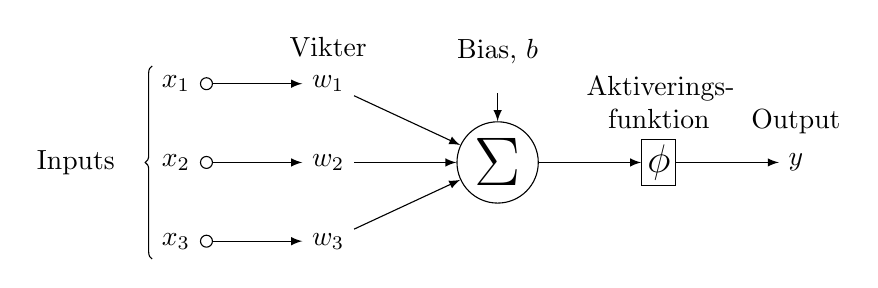
\begin{tikzpicture}[
			init/.style={draw,circle,inner sep=2pt,font=\Huge,join = by -latex},
		squa/.style={draw,inner sep=2pt,font=\Large,join = by -latex},
		start chain=2,node distance=13mm]
	\node[on chain=2] (x2) {$x_2$};
		\node[on chain=2,join=by o-latex] {$w_2$};
		\node[on chain=2,init] (sigma) {$\displaystyle\Sigma$};
		\node[on chain=2,squa,label=above:{\parbox{2cm}{\centering Aktiverings-\\ funktion}}] {$\phi$};
		\node[on chain=2,label=above:Output,join=by -latex] {$y$};
		\begin{scope}[start chain=1]
			\node[on chain=1] at (0,1.0cm) (x1) {$x_1$};
			\node[on chain=1,label=above:Vikter,join=by o-latex] (w1) {$w_1$};
		\end{scope}
		\begin{scope}[start chain=3]
			\node[on chain=3] at (0,-1.0cm) (x3) {$x_3$};
			\node[on chain=3,join=by o-latex] (w3) {$w_3$};
		\end{scope}
		\node[label=above:\parbox{2cm}{\centering Bias, $b$}] at (sigma|-w1) (b) {};
		\draw[-latex] (w1) -- (sigma);
		\draw[-latex] (w3) -- (sigma);
		\draw[-latex] (b) -- (sigma);
		\draw[decorate,decoration={brace,mirror}] (x1.north west) -- node[left=10pt] {Inputs} (x3.south west);
	\end{tikzpicture}
	\caption{Schematisk skiss över en neuron.}
	\label{fig:neuron}
\end{figure}

% Figur för sigmoidfunktionens graf
\begin{figure}
	\centering
	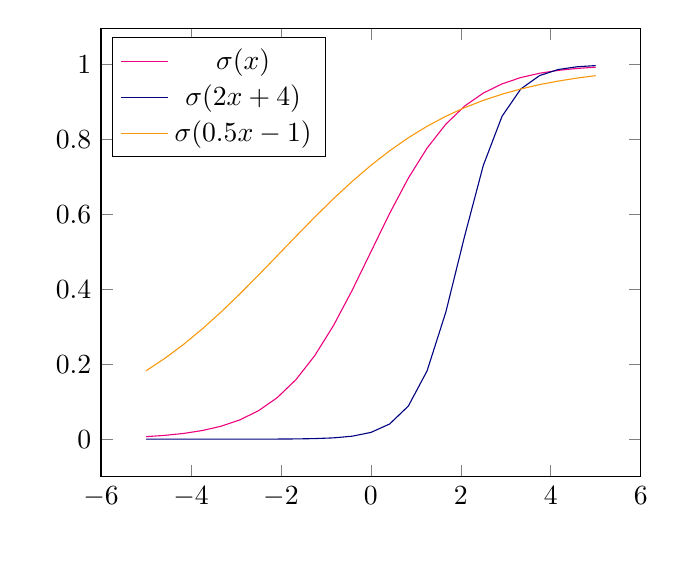
\begin{tikzpicture}
		\begin{axis}[legend style={at={(0.02,0.98)},anchor=north west},
			legend entries={$\sigma(x)$, $\sigma(2x + 4)$, $\sigma(0.5x - 1)$}]
			\addplot[RubineRed] {(1)/(1+e^-x)};
			\addplot[NavyBlue] {(1)/(1+e^(-2*x+4))};
			\addplot[YellowOrange] {(1)/(1+e^(-0.5*x-1))};
		\end{axis}
	\end{tikzpicture}
	\caption{Aktiveringsfunktionen sigmoid. \label{fig:sigmoid}}
\end{figure}

\subsection{Neuronnätsarkitektur}
\label{sec:arkitektur}
\noindent Neuronnät består av flera neuroner som alla är sammankopplade,
se figur~\ref{fig:network}.
I ett s.k. \textit{feed-forward} neuronnät får varje neuron inputs från
varenda neuron i det tidigare lagret.
Inputlagret får sina inputs direkt.
Det dolda lagret kallas så eftersom det inte är uppenbart hur det fungerar;
så vitt vi vet skulle det kunna använda sitt brutna ben
för att skyffla informationen framåt.
Outputlagrets aktiveringar blir resultatet av neuronnätet.
Medan antalet input- och outputneuroner otvetydligt kan bestämmas
från formen av ens träningsdata,
så finns bara empiriskt deriverad heuristik för strukturen på ens dolda lager.
Exempel på nackdelar med fler neuroner är längre träningstider
och behovet av mer träningsdata.
Neuronnät är specifika för en uppgift och en arkitektur som
fungerar bra i ett fall behöver inte nödvändigtvis göra det i ett annat.
\autocite{nielsen15}

% Figur för FF-nät
\begin{figure}
	\centering
	\def\layersep{2.5cm}
	\begin{tikzpicture}[shorten >=1pt,->,draw=black!50, node distance=\layersep]
		\tikzstyle{every pin edge}=[<-,shorten <=1pt]
		\tikzstyle{neuron}=[circle,fill=black!25,minimum size=17pt,inner sep=0pt]
		\tikzstyle{input}=[neuron, fill=red!45];
		\tikzstyle{output}=[neuron, fill=green!50];
		\tikzstyle{hidden neuron}=[neuron, fill=blue!50];
		\tikzstyle{annot} = [text width=4em, text centered]

		\foreach \name / \y in {1,...,2}
			\node[input, pin=left:Input \#\y] (I-\name) at (0,-\y) {};
		\foreach \name / \y in {1,...,3}
			\path[yshift=0.5cm]
				node[hidden neuron] (H-\name) at (\layersep,-\y cm) {};
		\node[output,pin={[pin edge={->}]right:Output}, right of=H-2] (O) {};
		\foreach \source in {1,...,2}
			\foreach \dest in {1,...,3}
				\path (I-\source) edge (H-\dest);
		\foreach \source in {1,...,3}
			\path (H-\source) edge (O);

		\node[annot,above of=H-1, node distance=1cm] (hl) {Dolt lager};
		\node[annot,left of=hl] {Inputlager};
		\node[annot,right of=hl] {Outputlager};
	\end{tikzpicture}
	\caption{Exempel på feed-forward neuronnät. \label{fig:network}}
\end{figure}

\textit{NARX-nät} (nonlinear autoregressive neural network with external input)
är ett neuronnät som kan tränas för att göra en tidsserieprediktion, alltså
förutsäga en tidsseries kommande datapunkter.
Genom att ha tillgång till tidigare datapunkter i serien,
\textit{feedback-input}, och en annan tidsserie, även kallad den externa
tidsserien.
NARX-nät lämpar sig följdaktligen till att felkompensera lutningsgivare;
uppgiften går ut på att förutsäga nästa datapunkt i serien och avgöra om den
stämmer in.\autocite{narxnet}
Att använda NARX-nät istället för feed-forward
kan vara en fördel när det gäller felkompensering. Feedforward kommer
inte ihåg vilken data den har stött på innan och den behandlar varje datapunkt
individuellt. Detta kan vara en fördel i vissa situationer men inte för felkompensering
av lutningsgivare då tidigare datapunkter hänger samman med varandra.
Fördelen med NARX-nät är att den kan komma ihåg tidigare värden och kan
anpassa sin output efter dem, vilket kan förenkla processen att förutsäga nästa värde.

\subsection{Stochastic gradient descent}
\label{sec:sdg}
% Förlustfunktionen
Med hjälp av en slät funktion för hur väl nätet approximerar träningsdatan
kan man korrelera små ändringar i vikter och biases
till små förbättringar i prestandan.
Den \emph{kvadratiska förlustfunktionen} är en sådan funktion:
\begin{equation} \label{eq:cost}
	C(w, b) \equiv \frac{1}{2n} \displaystyle\sum_x \lVert y(x) - a \rVert^2
\end{equation}
där $ w $ är alla vikter i nätet, $ b $ är alla biases,
$ n $ är antalet träningsindata, $ a $ är en vektor med utdata när $ x $ är indata
och summan är över all träningsindata $ x $.
Man ser att $ C(w, b) $ är icke-negativ då varje term i summan är positiv.
Dessutom är förlusten $ C(w, b) $ liten, det vill säga $ C(w, b) \approx 0 $,
när $ y(x) $ är ungefär lika med utdatan, $ a $, för alla träningsindata, $ x $.
Målet med träningsalgoritmen blir då att minimera $ C(w, b) $.

En algoritm för det är \emph{gradient descent}.
Om man föreställer sig en funktion $ f(x_1, x_2) $ som en dal,
se figur~\ref{fig:descent},
säger intuition att en boll skulle rulla nerför sluttningen till botten.
Vi kan simulera detta genom att räkna ut gradienten av $ f $.
Gradienten av $ f $, $ \nabla f $, vid en punkt är en vektor
som pekar i riktningen av den brantaste lutningen vid den punkten:
\begin{equation}
	\nabla f = \begin{bmatrix} \frac{\partial f}{\partial x_1} & \frac{\partial f}{\partial x_2} \end{bmatrix}^{T}
\end{equation}
där $ \partial f / \partial x_i $ är den partiella derivatan
som beskriver hur snabbt $ f $ växer med avseende på variablen $ x_i $.
Vi kan minska $ f $ genom att gå i riktningen av den negativa gradienten:
\begin{equation}
	x \leftarrow x - \eta \nabla f(x)
\end{equation}
där $ \eta $ är inlärningshastigheten,
en positiv skalär som bestämmer längden av steget.
Genom att generalisera det till flera dimensioner kan vi
applicera det på neuronnät:
\begin{align}
	w_k &\leftarrow w_k - \eta \frac{\partial C}{\partial w_k} \\
	b_l &\leftarrow b_l - \eta \frac{\partial C}{\partial b_l}
\end{align}

% Figur för gradient descent
\begin{figure}
	\centering
	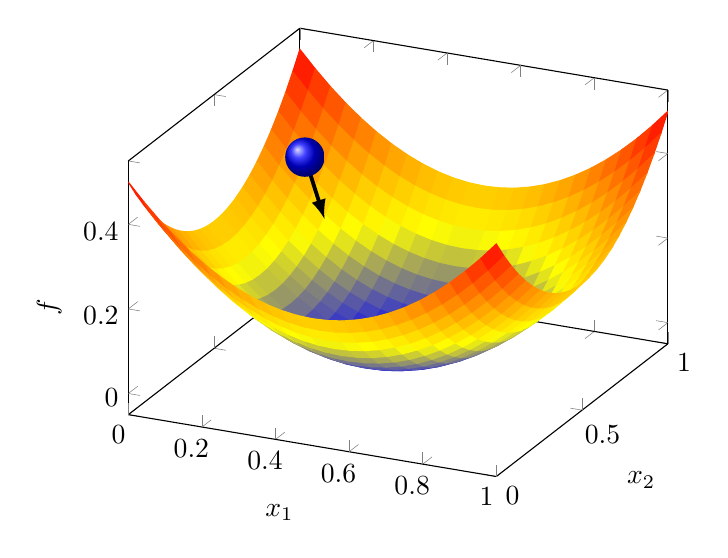
\begin{tikzpicture}
		\begin{axis}[domain=0:1,xlabel={$x_1$},ylabel={$x_2$},zlabel={$f$}]
			\addplot3[surf,shader=flat] {(x-0.5)^2 + (y-0.5)^2};
			\draw[->,line width=0.004\linewidth,>=latex] (axis cs:0.2,0.6,0.4) -- (axis cs:0.3,0.5,0.3);
			\node[circle,shading=ball,minimum width=0.5cm] (ball) at (axis cs:0.2,0.6,0.4) {};
		\end{axis}
	\end{tikzpicture}
	\caption{Gradient descent kan efterliknas vid en boll som rullar nerför en dal.}
	\label{fig:descent}
\end{figure}

Då förlustfunktionen i ekvation~\eqref{eq:cost} är ett genomsnitt av
förlusterna $ C_x = \frac{\lVert y(x) - a \rVert^2}{2} $ för individuella träningsexempel
kan det ta lång tid att beräkna gradienten med ett stort antal träningsindata.
\emph{Stochastic gradient descent} uppskattar $ \nabla C $ genom att
sampla en \emph{minibatch} av likformigt slumpade exempel
$ \mathbb{B} = \left\{ x_1, \dotsc, x_{m'} \right\} $ från träningsindatan
och räkna ut gradienten från dem:
\begin{equation}
	\nabla C \approx \frac{1}{m'} \sum^{m'}_{i=1} \nabla C_{x_i}
\end{equation}
med exempel från minibatchen $ \mathbb{B} $.
\autocite{goodfellow16,nielsen15}

\section{Syfte}
Syftet med undersökningen är att ta fram och utvärdera en algoritm med
artificiella neuronnät som felkompenserar lutningsgivare i elbussväxellådor.

%exempel på syfte: Syftet med undersökningen är att ta fram och utvärdera
%en algoritm och ett artificiellt neuronnät som båda felkompenserar lutningsivare i elbussväxellådor.

\section{Frågeställningar}
Vi vill undersöka\ldots
\begin{itemize}
% alternativ:	\item Varför råsignalen fårn lutningsgivaren och hastighetsmätaren blir opålitlig.
	\item Hur nätverket ska vara konfigurerat för att felkompensera; vilka inputs,
		outputs, typ av nät och antal neuroner och dolda lager?
% alternativ:	\item Hur ska algoritmen vara strukturerad för att felkompensera; vilka inputs,
%		beräkningar, metoder och antaganden [( tan(x)=x )] måste göras?
	\item Hur väl det fungerar att felkompensera med neuronnät?
% alternativ:	\item Hur väl det fungerar att felkompensera med neuronnät och algoritmer.
% 4/3: Detta är en generell fråga. Ska vi då besvara hur väl de fungerar generellt sett
% och specifikt då vi ger vårt resultat.
\end{itemize}


\section{Metod}

\definecolor{cb42e25}{RGB}{180,46,37}
\definecolor{ce94f2e}{RGB}{233,79,46}
\definecolor{cd2edf3}{RGB}{210,237,243}
\definecolor{c3f4340}{RGB}{63,67,64}
\definecolor{cadadad}{RGB}{173,173,173}

\begin{figure}
	\centering
	\begin{tikzpicture}[thick, >=stealth']
		\draw[<->] (5,0) node[below] {$s$} -| (0,3) node[right] {$h$};
		\draw[red, name path=slope] (0, 1) -- (1, 1) to[out=0,in=180] (4, 3) -- (5, 3);
		\path[name path=y] (1, 1) -- (3.6, 2.9);
		\path[name intersections={of=y and slope, by={A, B}}];
		\draw (A) -- (B); % Mark bus
		\coordinate (corner) at (A -| B);
		\draw[thin] (A) -| (B) ($ (corner) - (0.2, 0) $) |- ($ (corner) + (0, 0.2) $);

		\draw[thin, dashed] (A) -- (1, 0) node[below] {$s_1$} (A -| B) -- ({0, 0} -| B) node[below] {$s_1 + x$};
		\draw[decorate,decoration={brace,mirror,raise=3pt}] ({1, 1} -| B) -- node[right=4pt] {$\Delta h$} (B);
		\draw[decorate,decoration={brace,mirror,raise=23pt}] (B) -- (1, 1) node[midway, xshift=-19pt,yshift=26pt] {$l$};
		\draw pic[draw, "$v$", angle eccentricity=1.4] {angle=corner--A--B};
		\fill[draw=black,fill=white] (A) circle (2.0pt);

		\begin{scope}[shift={(1,1)},rotate=36,scale=0.0055]
			\path[fill=cb42e25] (259.9767,123.5489) ..
			controls (259.5847,123.5489) and (259.2486,123.6739) .. (258.9626,123.9290) ..
			controls (258.6776,124.1778) and (258.5337,124.5348) .. (258.5337,124.9938) ..
			controls (258.5337,125.3790) and (258.6716,125.7130) .. (258.9437,125.9880) ..
			controls (259.2187,126.2669) and (259.5507,126.4079) .. (259.9517,126.4079) ..
			controls (260.3497,126.4079) and (260.6877,126.2669) .. (260.9747,125.9958) ..
			controls (261.2547,125.7200) and (261.3967,125.3829) .. (261.3967,124.9938) ..
			controls (261.3967,124.5411) and (261.2547,124.1848) .. (260.9747,123.9329) ..
			controls (260.6877,123.6739) and (260.3557,123.5489) .. (259.9767,123.5489);
			\path[fill=ce94f2e] (373.3466,121.7386) ..
			controls (373.3466,121.7386) and (371.7726,129.0646) .. (366.3356,129.0646) --
			(10.3947,129.0646) .. controls (2.2927,129.0646) and (3.3829,121.7386) ..
			(3.3829,121.7386) -- (0.2341,84.8536) .. controls (0.2341,84.8536) and
			(0.2341,40.1426) .. (0.2341,26.4826) .. controls (0.2341,15.8967) and
			(8.2892,15.9088) .. (8.2892,15.9088) -- (358.9956,15.9088) .. controls
			(358.9956,15.9088) and (389.7196,12.8248) .. (389.7196,26.4826) .. controls
			(389.7196,40.1426) and (389.7196,57.4616) .. (389.7196,57.4616) --
			(373.3466,121.7386);
			\path[fill=cd2edf3] (368.4866,119.4046) -- (349.4186,119.4046) --
			(349.4186,69.3705) -- (384.2616,60.3476) -- (368.4866,119.4046);
			\path[fill=cd2edf3] (280.5166,121.3562) -- (16.5536,121.3562) --
			(9.2185,81.5245) -- (280.5166,81.5245) -- (280.5166,121.3562);
			\path[fill=c3f4340] (17.6720,20.9358) ..
			controls (17.6720,9.3494) and (27.0634,-1.9596) .. (38.6516,-1.9596) ..
			controls (50.2376,-1.9596) and (59.6296,9.3494) .. (59.6296,20.9358) ..
			controls (59.6296,32.5236) and (50.2376,41.9146) .. (38.6516,41.9146) ..
			controls (27.0634,41.9146) and (17.6720,32.5236) .. (17.6720,20.9358);
			\path[fill=cadadad] (26.5673,20.9358) ..
			controls (26.5673,14.2616) and (31.9766,8.8518) .. (38.6516,8.8518) ..
			controls (45.3226,8.8518) and (50.7346,14.2616) .. (50.7346,20.9358) ..
			controls (50.7346,27.6096) and (45.3226,33.0196) .. (38.6516,33.0196) ..
			controls (31.9766,33.0196) and (26.5673,27.6096) .. (26.5673,20.9358);
			\path[fill=c3f4340] (64.9016,20.9358) ..
			controls (64.9016,9.3494) and (74.2936,-1.9596) .. (85.8806,-1.9596) ..
			controls (97.4666,-1.9596) and (106.8596,9.3494) .. (106.8596,20.9358) ..
			controls (106.8596,32.5236) and (97.4666,41.9146) .. (85.8806,41.9146) ..
			controls (74.2936,41.9146) and (64.9016,32.5236) .. (64.9016,20.9358);
			\path[fill=cadadad] (73.7966,20.9358) ..
			controls (73.7966,14.2616) and (79.2066,8.8518) .. (85.8806,8.8518) ..
			controls (92.5516,8.8518) and (97.9636,14.2616) .. (97.9636,20.9358) ..
			controls (97.9636,27.6096) and (92.5516,33.0196) .. (85.8806,33.0196) ..
			controls (79.2066,33.0196) and (73.7966,27.6096) .. (73.7966,20.9358);
			\path[fill=c3f4340] (311.6096,20.10058) ..
			controls (311.6096,9.4194) and (320.10016,-1.10296) .. (332.5896,-1.10296) ..
			controls (344.1756,-1.10296) and (353.5676,9.4194) .. (353.5676,20.10058) ..
			controls (353.5676,32.5936) and (344.1756,41.9846) .. (332.5896,41.9846) ..
			controls (320.10016,41.9846) and (311.6096,32.5936) .. (311.6096,20.10058);
			\path[fill=cadadad] (320.5056,20.10058) ..
			controls (320.5056,14.3316) and (325.9146,8.9218) .. (332.5896,8.9218) ..
			controls (339.2606,8.9218) and (344.6726,14.3316) .. (344.6726,20.10058) ..
			controls (344.6726,27.6796) and (339.2606,33.896) .. (332.5896,33.896) ..
			controls (325.9146,33.896) and (320.5056,27.6796) .. (320.5056,20.10058);
			\path[fill=ce94f2e] (127.5966,24.7147) --
			(150.8966,24.7147) -- (150.8966,27.5487) -- (127.5966,27.5487) -- cycle;
			\path[fill=ce94f2e] (190.8836,24.7147) --
			(214.1844,24.7147) -- (214.1844,27.5487) -- (190.8836,27.5487) -- cycle;
		\end{scope}
	\end{tikzpicture}
	\caption{Lutningsberäkning: Ett visst värde på $x$ ger en rätvinklig triangel. \label{fig:fetbuss}}
\end{figure}

Bussen kördes med en GPS i bakre ändan för att få höjden som en funktion av sträckan.
I varje punkt kan en rätvinklig triangel konstrueras
där hypotenusan är bussens längd, se figur~\ref{fig:fetbuss}.
Då gäller Pythagoras sats:
\begin{equation} \label{eq:pythsats}
	x^2 + \Delta h^2 = l^2
\end{equation}
Genom att minimera en förlustfunktion av $x$
för hur väl ekvation~\ref{eq:pythsats} stämmer
beräknas lutningen $v$ med arcus tangens:
\begin{equation}
	v = \arctan \frac{\Delta h}{\min_x \left(l^2 - x^2 - \Delta h^2 \right)^2} \text{ där } 0 \leq x \leq l
\end{equation}

Bussen sattes i bruk då GPS och lutningsgivare mätte och loggade höjddata och
rå lutningsdata under bussfärden.
Efter bussfärden så beräknades lutningen i ekvation 10 
hjälp av höjddatan, en intergral av hastigheten och bussens längd.
Hastigheten deriverades och användes som neuronnätets träningsdata tillsammans med den
råa lutningsdatan och den beräknade lutningen.
Träningsdatan ska innefatta någorlunda varierade mätningar på både lutning och acceleration.

Med hjälp av MATLAB så tränades flera olika neurala nätverk med olika konfigurationer.
För att hitta den den bästa möjliga konfigurationen för lutningskorrigering tränades
olika cascade- och feedforward nätverk upp med olik mängd hidden layers, antal neuroner
i hidden layers och input layer.
Med den kvadratiska förlustfunktionen och gradient decent funktionen och så beräknades
optimala weights och biases för varje enskilt nätverk så alla neurala nätverk presterar
optimalt för just dess konfiguration.
Nätverken jämfördes och det nätverk som hade den minsta felmarginalen utvaldes som det
bästa nätverket med den bästa konfigurationen.
% Anders TODO
% Ska "fminbnd" funktionen och " h2 = interp1(s, h, s1 + x)" förklaras här?
%[Skriv in ett specifikt antal neruala nätverk som tränades upp (görs efter projektveckan) (eller blir det bättre att inte ha ett specifikt antal?)]
%Såg att det fanns ingen bakgrund om cascadeforward - Ska vi bara testa feedforward nätverk?
%Hur mycket tid ska vi ge ett nätverk att träna? 1, 10, 40 min? Detta beror väl på hur snabbt de tränas och hur snabbt de närmar sig det optimala. Säg 180 min / antal nätverk = träningstid för ett nätverk ? Antar att vi kan bestämma vad som är rimligt på projektveckan.
%   OBS!_-_-_-_-_-_-_-_-_Hur ska vi jämföra dem objektivt?_-_-_-_-_-_-_-_-_-_  Vi skulle kunna beräkna den absoluta intergralen mellan nätverkets output och den riktiga lutningen och välja det nätverk som får det lägsta värdet (är detta rimligt/möjligt?). Om vi endast tränar ca 20st så är väl det möjligt att jämflöra dem för hand.
%Ska ett mer passande ord än 'optimal' användas då det är inte helt optimalt i sig, utan de är de bästa vi kunde hitta?


\section{Resultat}

% Resultat från lutningsgivare
\begin{sidewaysfigure}
	\centering
	\begin{tikzpicture}
		\begin{groupplot}[
				width = \textwidth, height = \textheight / 2,
				no markers,
				x unit = s, xlabel = Tid,
				y unit = \%, ylabel = Lutning,
				enlarge x limits = false,
				enlarge y limits = {abs = 0.1cm},
				group style = {
					group size = 1 by 2,
					vertical sep = 0pt,
					x descriptions at = edge bottom,
				},
				% Add a zero line
				extra y ticks=0, extra y tick labels=, extra y tick style={grid=major},
				extra x tick style = {grid = major},
				extra x tick labels=,
				extra x ticks= {59.94, 102.18, 122.8, 154.74, 214.72, 228.9},
				]
				\pgfplotstableread{phi.dat}\phidata;
				\nextgroupplot
				\addplot table[x=Time, y=phi] from \phidata;
				\addlegendentry{$\phi$}
				\addplot[dashed, color = DarkRed] table[x=Time, y expr = 100 * \thisrow{a} / 9.81] from \phidata;
				\addlegendentry{$\frac{a}{g}$}
				\nextgroupplot
				\addplot[color = Emerald] table[x=Time, y = y] from \phidata;
				\addlegendentry{$y$}
		\end{groupplot}
	\end{tikzpicture}
	\caption{$\phi$ och $\frac{a}{g}$ som funktioner av tiden konkatenerade från 7 loggar och kontrasterade mot den beräknade lutningen från Gps:en. \label{fig:phiresult}}
\end{sidewaysfigure}

\begin{figure}
	\centering
	\begin{tikzpicture}
		\begin{axis}[
				no markers,
				legend style={at={(0.02,0.98)},anchor=north west},
				table/x expr=2 * 0.02 * 10 * \coordindex,
				xlabel = Tid, x unit = s,
				ylabel = Lutning, y unit = \%,
				]
				\addplot table[y=a] from {predict7.dat};
				\addlegendentry{$a$}
				\addplot table[y=y] from {predict7.dat};
				\addlegendentry{$y$}
		\end{axis}
	\end{tikzpicture}
	\caption{Neuronnätets beräknade lutning gentemot Gps:ens lutning. \label{fig:netresult}}
\end{figure}

% Hur väl det fungerar att felkompensera?
Den kvadratiska förlusten blev \num[round-precision=3]{0.002055976870427035}
vilket motsvarar en genomsnittllig avvikelse på
\SI[round-precision=3]{2.7205728686321}{\percent}.
% Hur nätverket ska vara konfigurerat?
%5hidden 4 feedback dealy 0,3 learing rate (eta) 10 batch size
Vi fick lägst förlust när vi tränade ett narxnät med följande parametrar:
\SI{5}{\styck} neuroner i hidden layer, \SI{4}{\styck} senaste värdena i feedback delay,
\num{0.3} $\eta$ (learning rate) och minibatchens kardinalitet på \num{10}.

I figur~\ref{fig:phiresult} kontrasteras den beräknade lutningen, $y$, med den
uppmätta lutningen, $ \phi - \frac{a}{g} $, och rådatan från
lutningsgivaren, $phi$.
I både figur~\ref{fig:phiresult} och figur~\ref{fig:netresult}
innebär positiv och negativ lutning att bussen körs uppför respektive
nedför en lutning som är angiven i procent.

Figur~\ref{fig:netresult} visar neuronnätets aktiveringar som tar in
lutningsgivarens råvärde och bussens acceleration
och ger lutningen som neuronnätet beräknat, $a$.
Denna visas med den beräknade lutingen från Gps:en, $y$.


\section{Diskussion \& slutsatser}

\clearpage
\printbibliography
\end{document}
